\documentclass[a4paper,11pt]{article}

\usepackage[T1]{fontenc}
\usepackage[utf8]{inputenc}
\usepackage[french,german,english]{babel}


%%%%%%%%%%%%%%%%%%%%%%%%%%%%%%%%%%%%%%%%%%%%%%%
% UVIGO THESIS TEMPLATE:
%  Variant 1.0 -> Latin modern, large text width&height
%\usepackage{lmodern}
%\usepackage[a4paper,top=22mm,bottom=28mm,inner=35mm,outer=25mm]{geometry}
%
%  Variant 2.0 -> Utopia, Gabarrit A (lighter pages)
%\usepackage{fourier} 
%\usepackage[adobe-utopia]{mathdesign}

\setlength{\textwidth}{146.8mm}
\setlength{\oddsidemargin}{11.6mm}
\setlength{\evensidemargin}{0.8mm}
\setlength{\topmargin}{-2.2mm}
\setlength{\textheight}{221.9mm}
\setlength{\headheight}{14pt}
\setlength{\parindent}{0pt}

\usepackage{setspace} % increase interline spacing slightly
\setstretch{1.1}

\makeatletter
\setlength{\@fptop}{0pt}  % for aligning all floating figures/tables etc... to the top margin
\makeatother

\usepackage{graphicx}
\usepackage[table]{xcolor}
\graphicspath{{images/}}

\usepackage{subfigure}
\usepackage{booktabs}
\usepackage{microtype}
\usepackage{url}
\usepackage[final]{pdfpages}

\usepackage{fancyhdr}
\renewcommand{\sectionmark}[1]{\markright{\thesection\ #1}}
\pagestyle{fancy}
	\fancyhf{}
	\renewcommand{\headrulewidth}{0.4pt}
	\renewcommand{\footrulewidth}{0pt}
	\fancyhead[OR]{\bfseries \nouppercase{\rightmark}}
	\fancyhead[EL]{\bfseries \nouppercase{\leftmark}}
	\fancyfoot[EL,OR]{\thepage}
\fancypagestyle{plain}{
	\fancyhf{}
	\renewcommand{\headrulewidth}{0pt}
	\renewcommand{\footrulewidth}{0pt}
	\fancyfoot[EL,OR]{\thepage}}
\fancypagestyle{addpagenumbersforpdfimports}{
	\fancyhead{}
	\renewcommand{\headrulewidth}{0pt}
	\fancyfoot{}
	\fancyfoot[RO,LE]{\thepage}
}

\usepackage{listings}
\lstset{language=[LaTeX]Tex,tabsize=4, basicstyle=\scriptsize\ttfamily, showstringspaces=false, numbers=left, numberstyle=\tiny, numbersep=10pt, breaklines=true, breakautoindent=true, breakindent=10pt}

\usepackage{hyperref}
\hypersetup{pdfborder={0 0 0},
	colorlinks=true,
	linkcolor=black,
	citecolor=black,
	urlcolor=black}
\urlstyle{same}

\makeatletter
\def\cleardoublepage{\clearpage\if@twoside \ifodd\c@page\else
    \hbox{}
    \thispagestyle{empty}
    \newpage
    \if@twocolumn\hbox{}\newpage\fi\fi\fi}
\makeatother \clearpage{\pagestyle{plain}\cleardoublepage}


%%%%% CHAPTER HEADER %%%%
\usepackage{color}
\usepackage{tikz}
\usepackage[explicit]{titlesec}
\newcommand*\chapterlabel{}
\titleformat{\chapter}[display]
	{\normalfont\bfseries\Huge}
	{\gdef\chapterlabel{\thechapter\ }}
 	{0pt}
 	  {\begin{tikzpicture}[remember picture,overlay]
    \node[yshift=-8cm] at (current page.north west)
      {\begin{tikzpicture}[remember picture, overlay]
        \draw[fill=gray] (0,0) rectangle(35.5mm,15mm);
        \node[anchor=north east,yshift=-7.2cm,xshift=34mm,minimum height=30mm,inner sep=0mm] at (current page.north west)
        {\parbox[top][30mm][t]{15mm}{\raggedleft $\phantom{\textrm{l}}$\color{white}\chapterlabel}};
        \node[anchor=north west,yshift=-7.2cm,xshift=37mm,text width=\textwidth,minimum height=30mm,inner sep=0mm] at (current page.north west)
              {\parbox[top][30mm][t]{\textwidth}{\color{black}#1}};
       \end{tikzpicture}
      };
   \end{tikzpicture}
   \gdef\chapterlabel{}
  }

\titlespacing*{\chapter}{0pt}{50pt}{30pt}
\titlespacing*{\section}{0pt}{13.2pt}{*0}
\titlespacing*{\subsection}{0pt}{13.2pt}{*0}
\titlespacing*{\subsubsection}{0pt}{13.2pt}{*0}

\newcounter{myparts}
\newcommand*\partlabel{}
\titleformat{\part}[display]
	{\normalfont\bfseries\Huge}
	{\gdef\partlabel{\thepart\ }}
 	{0pt}
 	  {\setlength{\unitlength}{20mm}
	  \addtocounter{myparts}{1}
	  \begin{tikzpicture}[remember picture,overlay]
    \node[anchor=north west,xshift=-65mm,yshift=-6.9cm-\value{myparts}*20mm] at (current page.north east)
      {\begin{tikzpicture}[remember picture, overlay]
        \draw[fill=black] (0,0) rectangle(62mm,20mm);
        \node[anchor=north west,yshift=-6.1cm-\value{myparts}*20mm,xshift=-60.5mm,minimum height=30mm,inner sep=0mm] at (current page.north east)
        {\parbox[top][30mm][t]{55mm}{\raggedright \color{white}Part \partlabel $\phantom{\textrm{l}}$}};
        \node[anchor=north east,yshift=-6.1cm-\value{myparts}*20mm,xshift=-63.5mm,text width=\textwidth,minimum height=30mm,inner sep=0mm] at (current page.north east)
              {\parbox[top][30mm][t]{\textwidth}{\raggedleft \color{black}#1}};
       \end{tikzpicture}
      };
   \end{tikzpicture}
   \gdef\partlabel{}
  }

\usepackage{amsmath,amsfonts,amsthm}

% Predefined theorem-like environments
\newtheorem{theorem}{Theorem}[section]
\newtheorem{remark}{Remark}[section]

% Fix the problem with delimiter size caused by fourier and amsmath packages.
\makeatletter
\def\resetMathstrut@{%
  \setbox\z@\hbox{%
    \mathchardef\@tempa\mathcode`\(\relax
      \def\@tempb##1"##2##3{\the\textfont"##3\char"}%
      \expandafter\@tempb\meaning\@tempa \relax
  }%
  \ht\Mathstrutbox@1.2\ht\z@ \dp\Mathstrutbox@1.2\dp\z@
}
\makeatother

\usepackage{IEEEtrantools}

\usepackage{graphicx}
\usepackage{grffile}
\usepackage[left=2cm,right=2cm,top=2cm,bottom=2cm]{geometry}

%\hypersetup{pageanchor=false}

\begin{document}
\begin{titlepage}

\Large
\sffamily

\begin{center}
  \begin{tabular}{c}
    
\includegraphics[width=0.55\textwidth]{./images/unilogo}
  \end{tabular}
\end{center}

\vfill
\begin{center}
  \huge 
    {\huge Desarrollo de una ensamblador para ARM/THUMB}

\vspace{24pt}
\textcolor{gray}{\small{}}
\end{center}

\vspace*{2cm}
\centerline{{\huge Johan Sebastián Villamarín Caicedo}}

\vfill

\begin{center}
{\large
  Trabajo de Fin de Grado \\
  Escuela de Ingeniería de Telecomunicación \\
  Grado en Ingeniería de Tecnologías de Telecomunicación
}
\end{center}

\vfill
\begin{center}{
{   Tutor \\
    Martín Llamas Nistal
}
}
\end{center}
\vfill
\centerline{\fontsize{11}{13.8} \selectfont Curso 2021/2022}
\end{titlepage}

\newpage
\tableofcontents
\listoffigures
\setcounter{page}{1}


\newpage
\section{Introducción}
{
    Hoy en día la programación es cada vez una competencia más demandada, con la automatización de tareas siempre surge la necesidad de un software ya sea específico o no. \\

    Debido a esto cada vez obtienen mas interés los estudios relacionados con cualquier tipo de desarrollo software (WEB, Android, etc). Entre los distintos lenguajes de programación están los conocidos como \textbf{de bajo nivel o ensamblador}. En estos el programador tiene pleno control sobre los registros de la cpu, habiendo uno específico para cada arquitectura y soportado solo por esta. \\
    
    Por ello se usa comunmente simuladores para el desarrollo sin necesidad de tener el hardware o incluso en la docencia de este tipo de lenguajes. Permitiendo estos escribir y probar código para una arquitectura que no es la del equipo. Sin embargo, estos simuladores pueden depender de librerías de terceros o programas por lo que su instalación y uso puede no ser siempre tan rápida. Además no todos son intuitivos y/o configurables. \\
    
    Como solución a todo esto, y para el caso concreto de ARM Thumb, se decide desarrollar un \textbf{Ensamblador y Simulador Web para ARM/THUMB}. Al tratarse de una plataforma web simplificamos enormemente la instalación dado que bastaría con disponer de cualquier navegador y conexión a internet. Además esto hace que se pueda usar desde cualquier sistema operativo. \\

    Las tecnologías empleadas para esta plataforma son:
    \begin{enumerate}
        \item \textbf{React}: JavaScript Framework
        \item \textbf{NodeJS}: JavaScript Engine
        \item \textbf{TypeScript}: React - TypeScript
        \item \textbf{React-Redux}
        \item \textbf{Docker}
    \end{enumerate}
}

\section{Objetivos}
{
    El objetivo principal de este trabajo es crear una plataforma web en la que los usuarios puedan escribir código en lenguaje ARM/THUMB, compilar y probar el programa de forma interactiva. Pudiendo ver en todo momento el estado de la CPU, sus registros y flags de estado, así como la memoria y su contenido. \\
    
    Módulos de la aplicación web:
    \begin{enumerate}
        \item \textbf{Editor de código}: Editor de texto con soporte para ARM/Thumb con syntax highlighting.
        \item \textbf{Visualizador de registros}: Panel con los registros de la CPU y su valor. Así como el estado de los flags.
        \item \textbf{Visualizador de programa}: Lista de instrucciones ensamblador que el usuario ha cargado a la CPU.
        \item \textbf{Visualizador de memoria}: Panel con la memoria de la CPU.
        \item \textbf{ARM Help}: Mínima ayuda sobre las instrucciones ARM disponibles en el simulador.
    \end{enumerate}
    
    Como objetivo adicional se busca que la aplicación se lo mas intuitiva posible y ofrezca control absoluto sobre la CPU y la memoria que se está simulando. Con facilidades para modificar los valores de los registros o de la memoria.
}

\section{Resultados}
Plataforma web integrando un ensamblador y simulador para ARM Thumb.

    \subsection{ARM Thumb Emulator}
    {
        Módulo en TypeScript con todas las funciones necesarias para la simulación de código escrito en ARM/THUMB.
        Este módulo se desarrolló de forma separada para su posterior integración en el sistema final. Gracias a esta división también se realizaron pruebas unitarias de cada instrucción implementada para asegurar que el comportamiento del simulador es el esperado si se ejecutase en una CPU de ARM real.
    
        \begin{figure}[h]
         \centering
            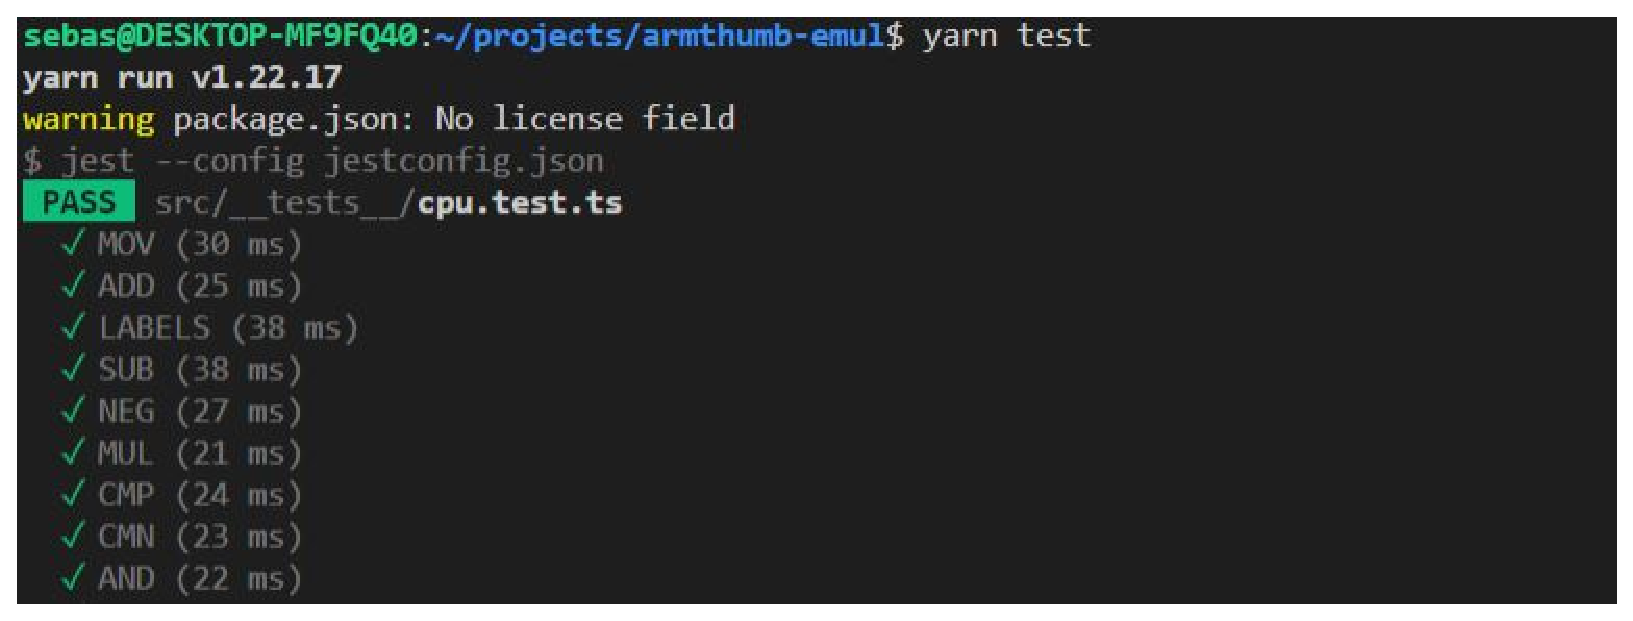
\includegraphics[width=0.85\textwidth]{images/tests}
            \caption{Running Test Suite}
        \end{figure}
        
        \begin{figure}[h]
         \centering
            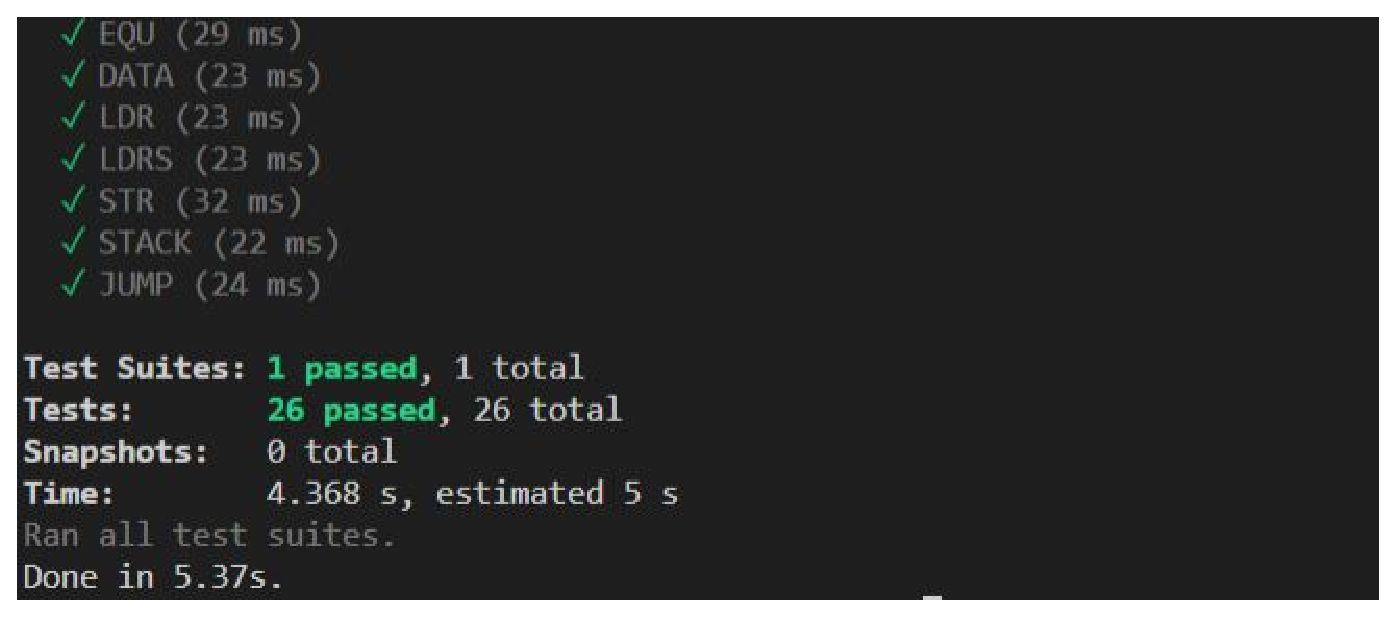
\includegraphics[width=0.85\textwidth]{images/tests2}
            \caption{Finished Test Suite}
        \end{figure}
        
        Para cada test hay un código de ARM/Thumb cuyo resultado es conocido y siempre el mismo. De este modo podemos asegurar que todo sigue funcionando como debe tan solo con ejecutar las pruebas unitarias.
        
        El estado de la CPU tras la ejecución del código es volcado a un archivo temporal (add.json.tmp) de no existir. De este modo si el estado es correcto basta con eliminar la extensión .tmp para que en los siguientes tests este sea el estado esperado de la CPU.
        
        \begin{figure}[h]
         \centering
            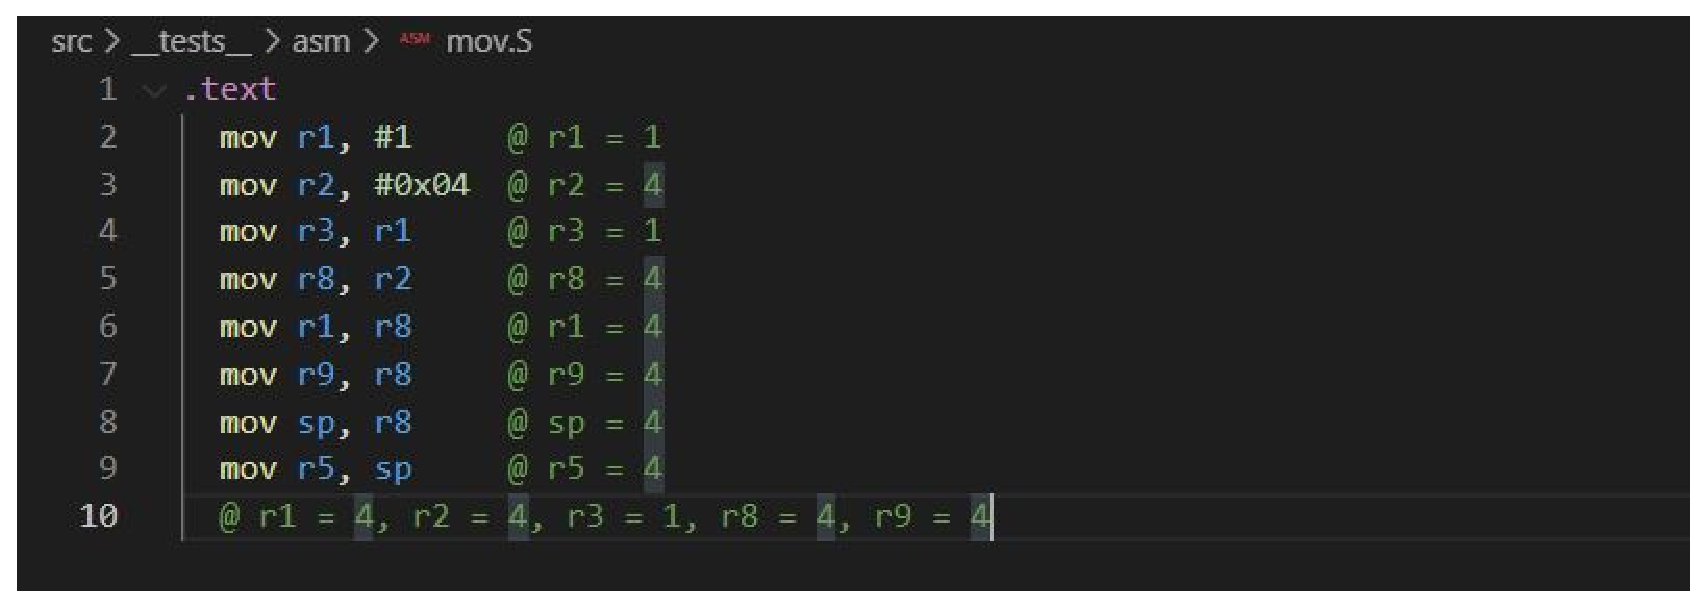
\includegraphics[width=0.85\textwidth]{images/asm}
            \caption{ARM Test Code}
        \end{figure}
    
        \begin{figure}[h]
         \centering
            \includegraphics[width=0.85\textwidth]{images/state}
            \caption{CPU Expected State}
        \end{figure}
        
        Cada test simboliza una instrucción en ARM Thumb, salvo en algunos casos donde se prueban variantes de una sola en un mismo test (ldr, ldrb, ldrh). Cada test tendrá su correspondiente archivo con el estado esperado de la cpu con el que se comprobará que la ejecución sea correcta.

        \newpage
        La CPU emulada es básicamente un objeto de javascript con los registros, flags, memoria y todas las funciones necesarias para compilar y ejecutar el código. \\

        \begin{figure}[h]
         \centering
            
\includegraphics[width=0.85\textwidth, height=0.55\textwidth]{images/cpu}
            \caption{ARM CPU Type}
        \end{figure}

        Para inicializar la cpu basta con llamar a la función defaultCPU() que exporta el módulo. Esta función devuelve un objeto cpu con los valores por defecto, se puede modificar el tamaño de la memoria y del stack por parámetros.
    }
    
    \newpage
    \subsection{Web Interface}
    {
        Como interfaz de usuario se desarrolla una plataforma web que integra el emulador. Desarrollada en TypeScript con el framework React. Gracias a la librería React-Redux se comparte un estado global a todos los componentes de la interfaz. Este estado consta de:
        \begin{enumerate}
            \item \textbf{cpu}: El objeto CPU del emulador.
            \item \textbf{assembly}: El código ensamblador que el usuario ha introducido.
            \item \textbf{error}: Mensaje de error para mostrar en la interfaz, en caso de haber error.
        \end{enumerate}

        Este estado es utilizado por los distintos componentes de la interfaz para mantener siempre la información que se muestra actualizada.
        
        \begin{figure}[h]
         \centering
            \includegraphics[width=0.85\textwidth]{images/ui}
            \caption{User Interface}
        \end{figure}
        
        \subsubsection{Code Editor}
        {
            Editor de texto con highlighting para ARM Thumb. Hace uso de React CodeMirror que tiene soporte para distintos lenguajes. En este caso se extiende la librería para soportar ARM Thumb. Además incorpora múltiples atajos de teclado para mover, cortar o seleccionar texto.
            
            \begin{figure}[h]
                \centering
                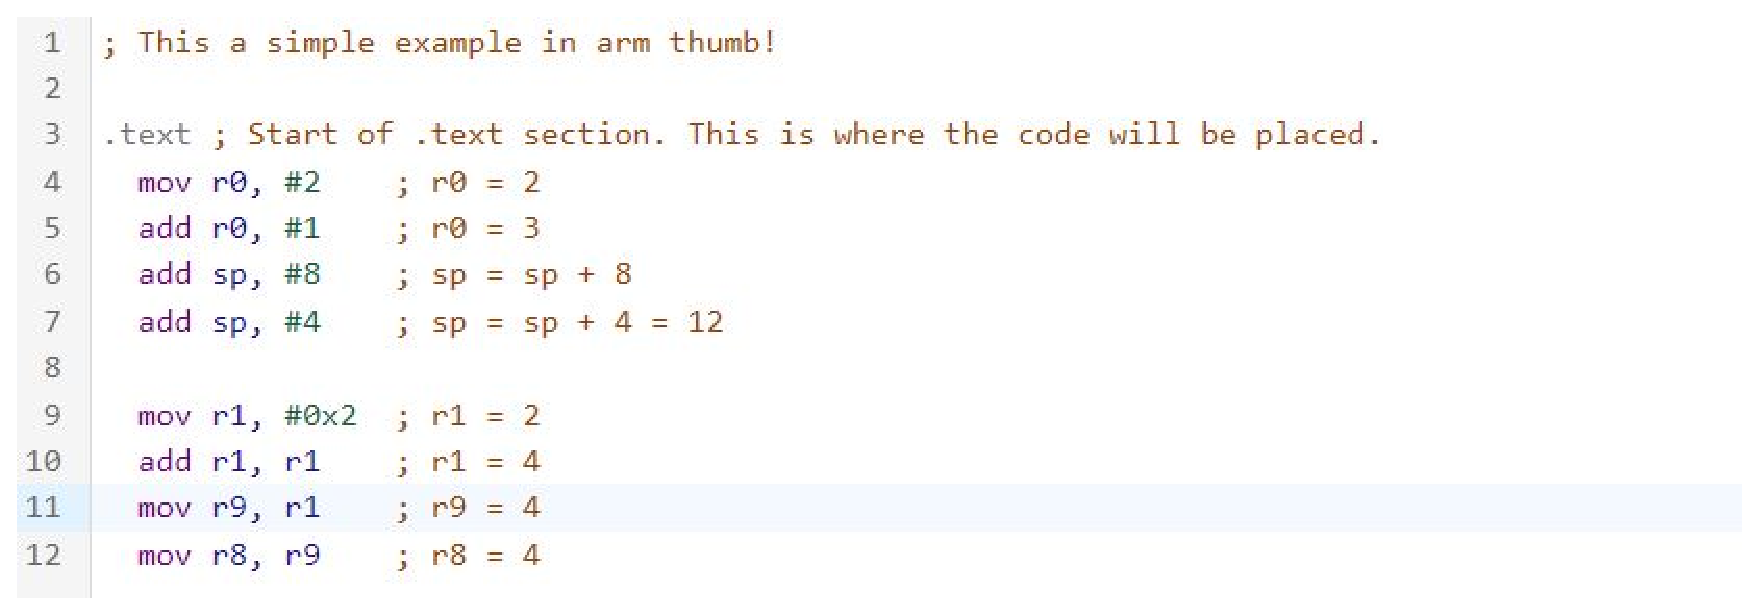
\includegraphics[width=0.85\textwidth]{images/editor}
                \caption{ARM Code Editor}
            \end{figure}

            Este componente muestra en todo momento el valor de \textbf{assembly} del estado de la aplicación y es el encargado de actualizarlo con la entrada del usuario.
            Una vez escrito el programa el usuario puede cargarlo en la CPU mediante el botón de \textbf{Load Program} en la parte superior de la interfaz. \\

            \begin{figure}[h]
                \centering
                \includegraphics[width=0.85\textwidth]{images/compiled}
                \caption{Compiled Code}
            \end{figure}

            \newpage
            De haber algún error en el código se notificaría al usuario a través de un PopUp indicando la causa y la línea del error.

            \begin{figure}[h]
                \centering
                \includegraphics[width=0.85\textwidth]{images/compilererror}
                \caption{Error Compiling Code}
            \end{figure}
        }
        
        \subsubsection{Programa}
        {
            Una vez cargado el programa este estará en el panel izquierdo, donde se podrá ver la siguiente instrucción a ejecutar,
            los breakpoints del programa así como todas las demás instrucciones cargadas en la CPU. \\
            
            \begin{figure}[h]
                \centering
                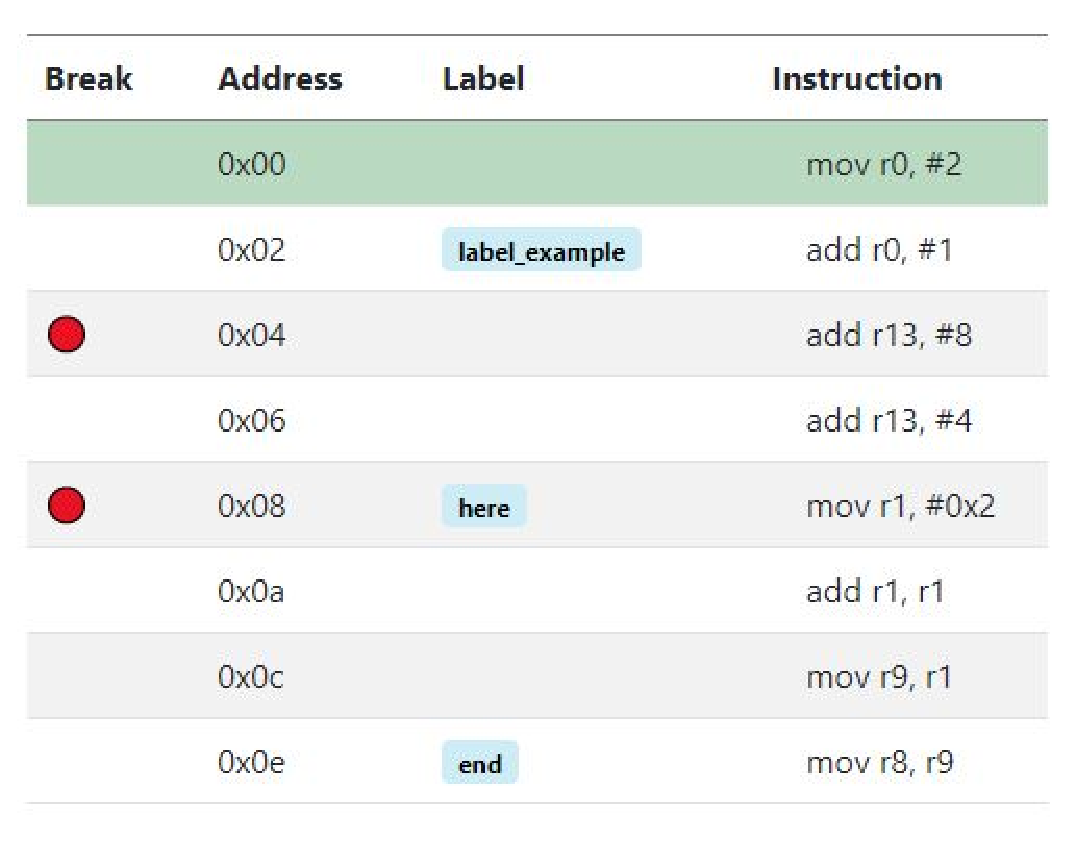
\includegraphics[width=0.8\textwidth, height=0.35\textheight]{images/programa}
                \caption{Loaded Program}
            \end{figure}
            
            Además se pueden poner/quitar breakpoints con un simple click.
            Del mismo modo para ejecutar el programa tras su carga tenemos dos botones:
            \begin{enumerate}
                \item \textbf{Run Code}: Ejecuta todo el código cargado en la CPU.
                \item \textbf{Step Into}: Ejecuta instrucción a instrucción el programa cargado.
            \end{enumerate}
        }

        \subsubsection{Registros y flags}
        {
            En ARM Thumb tenemos acceso a 16 registros, la mitad conocidos como \textbf{Low Registers} y la mitad superior \textbf{High Registers}.
            Estos registros están siempre representados en pantalla junto con los flags de la CPU. 

            Los registros inferiores son los del 0 al 7, mientras que los superiores son del 8 al 15.
            Algunos de los registros superiores son registros con un propósito específico. Estos son:
            \begin{enumerate}
                \item \textbf{R13 (SP)}: Stack Pointer. Se actualiza automáticamente al hacer push o pop
                \item \textbf{R14 (LR)}: Long Return Register.
                \item \textbf{R15 (PC)}: Program Counter Register. Se actualiza automáticamente con la dirección de la próxima instrucción
            \end{enumerate}

            \begin{figure}[h]
                \centering
                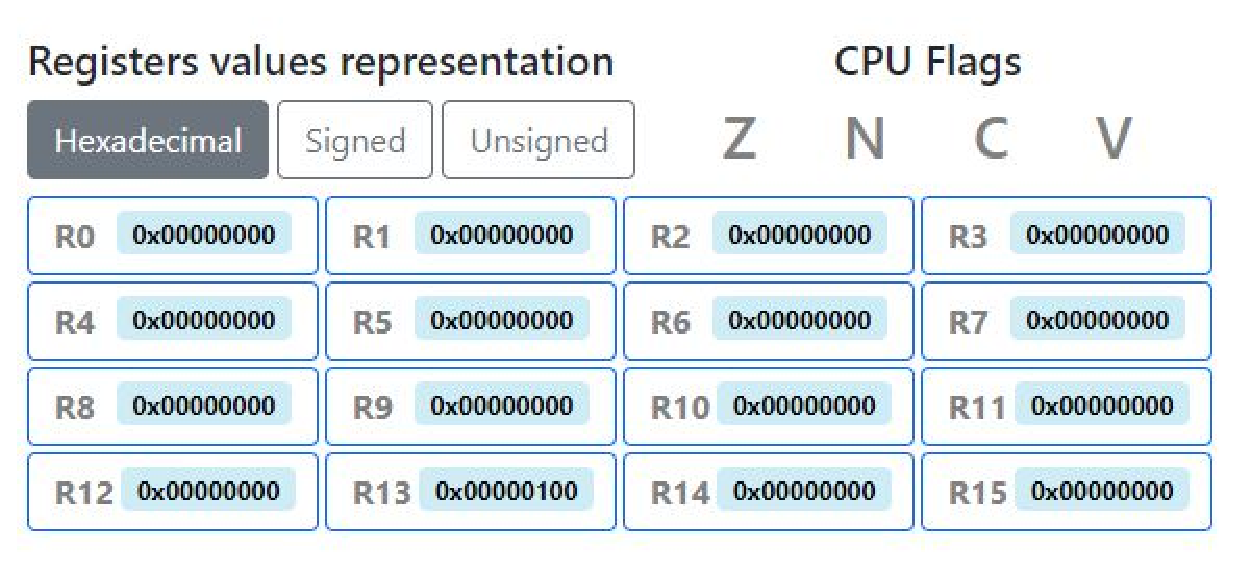
\includegraphics[width=0.85\textwidth]{images/registers}
                \caption{Registers Menu}
            \end{figure}

            Como se puede ver en la figura 11 cada registro aparece por defecto en formato hexadecimal.
            Además se puede cambiar el formato entre hexadecimal, signed y unsigned con un simple click.

            El valor de cada registro puede ser modificado en cualquier momento. Clickando en el registro
            que queremos cambiar abriremos un menú de modificación donde podremos ver el valor actual en
            todos los formatos disponibles así como introducir un nuevo valor.

            \begin{figure}[h]
                \centering
                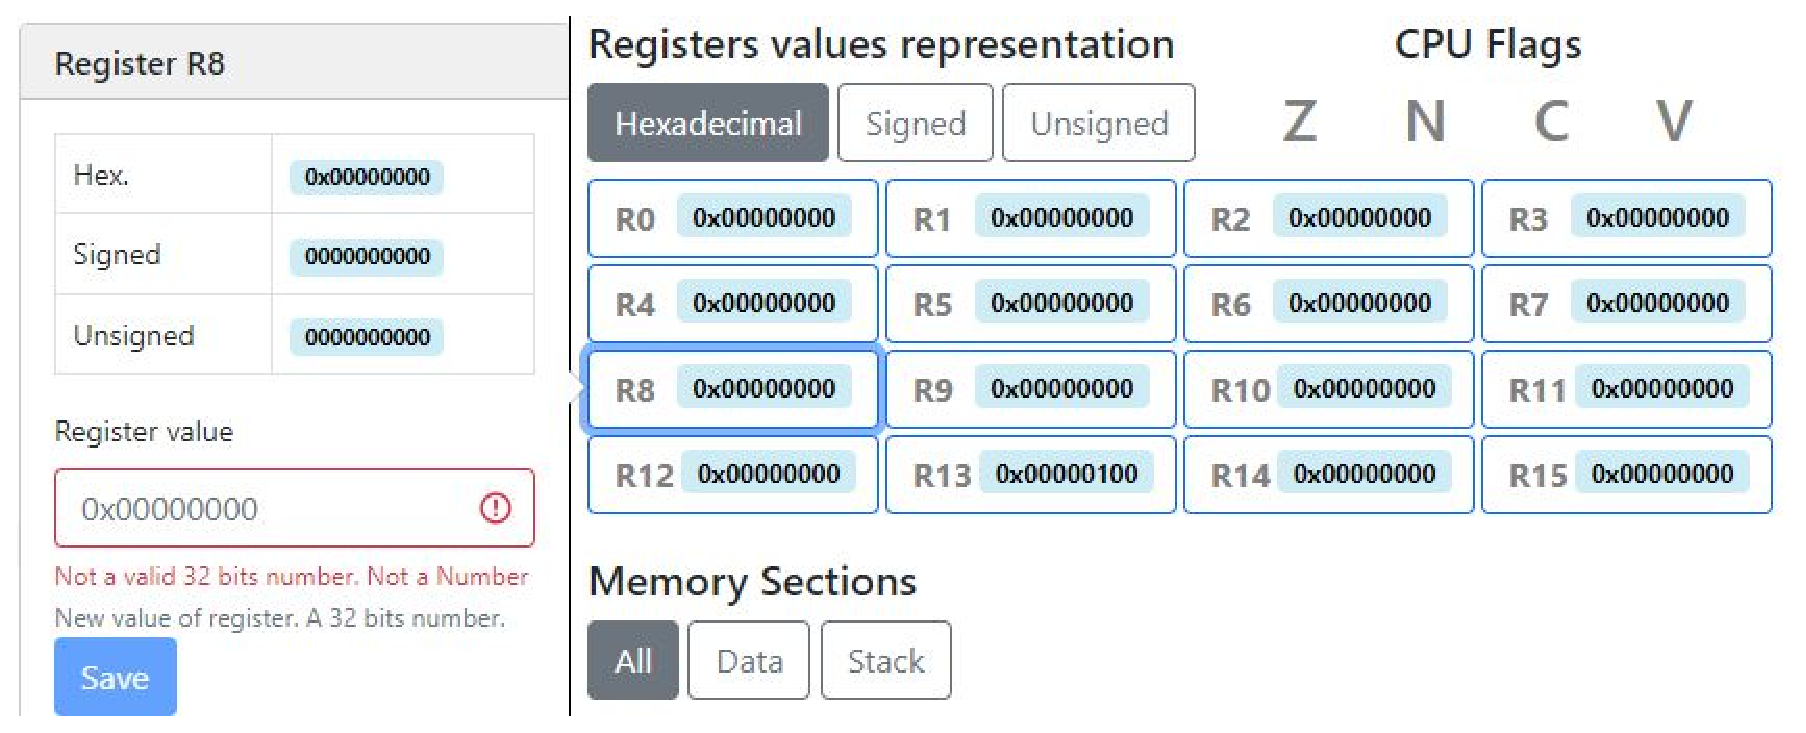
\includegraphics[width=0.85\textwidth]{images/modifyregister}
                \caption{Change Register Value}
            \end{figure}

            Además se comprueba en todo momento que la entrada del usuario sea un nº de 8 bits válido.
            Ya sea en formato hexadecimal o decimal, no se admiten números negativos, y se habilita el botón
            de guardar solo si la entrada es correcta.

            En la parte superior derecha tenemos los flags de la CPU. Estos flags se activan en algunas operaciones
            como las de comparar dependiendo del resultado de dicha operación. En caso de ejecutar el programa sin ir
            paso a paso el estado de los flags sería siempre el que hay al final de la ejecución, 
            igual que los registros.

            \begin{figure}[h]
                \centering
                \includegraphics[width=0.85\textwidth]{images/flags}
                \caption{Flags Example}
            \end{figure}

            En este ejemplo se compara r0 con un 3. Al ser la comparación una resta y dar esta cero se activa
            el flag correspondiente Z. Los distintos flags son:
            \begin{enumerate}
                \item \textbf{Z}: Resultado igual a 0
                \item \textbf{N}: Resultado negativo
                \item \textbf{C}: Bit de acarreo
                \item \textbf{V}: Overflow con signo
            \end{enumerate}
        }

        \newpage
        \subsubsection{Memoria}
        {
            Debajo de los registros está la memoria de la CPU, se inicializa por defecto a 64 palabras (4 bytes)
            como zona libre y 64 más para el stack. Se puede visualizar toda la memoria a la vez, sólo la zona de datos o sólo el stack.

            \begin{figure}[h]
                \centering
                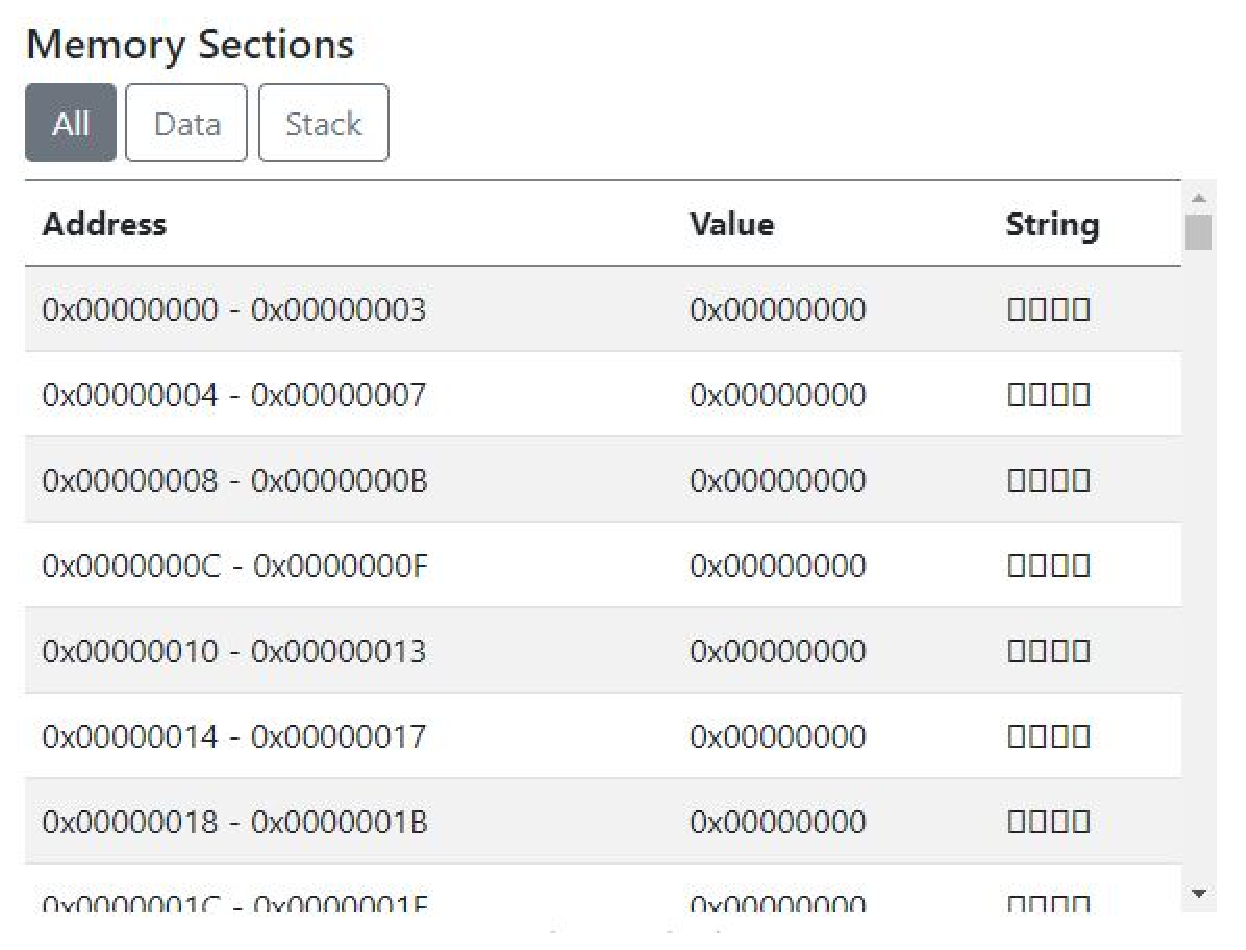
\includegraphics[width=0.85\textwidth]{images/memory}
                \caption{Memory Menu}
            \end{figure}

            El usuario puede utilizar directivas de ensamblador para inicializar la memoria
            con cualquier valor que necesite durante la ejecución. En caso de que el programa necesite más memoria de la disponible esta crece de forma automática, esto puede pasar
            en operaciones como push o en programas que soliciten guardar muchos datos iniciales.

            \begin{figure}[h]
                \centering
                \includegraphics[width=0.85\textwidth]{images/memorydata}
                \caption{Memory Data Example}
            \end{figure}
            Como se puede ver en este ejemplo hay diferentes directivas para almacenar desde strings, bytes, medias palabras
            o palabras. Así como directivas para alinear el próximo dato.

            Además del mismo modo que para los registros los valores de la memoria son fácilmente modificables,
            para ello basta con clickar en la zona de memoria cuyo valor deseamos modificar y se nos abrirá un menú similar al visto
            para modificar un registro.

            \begin{figure}[h]
                \centering
                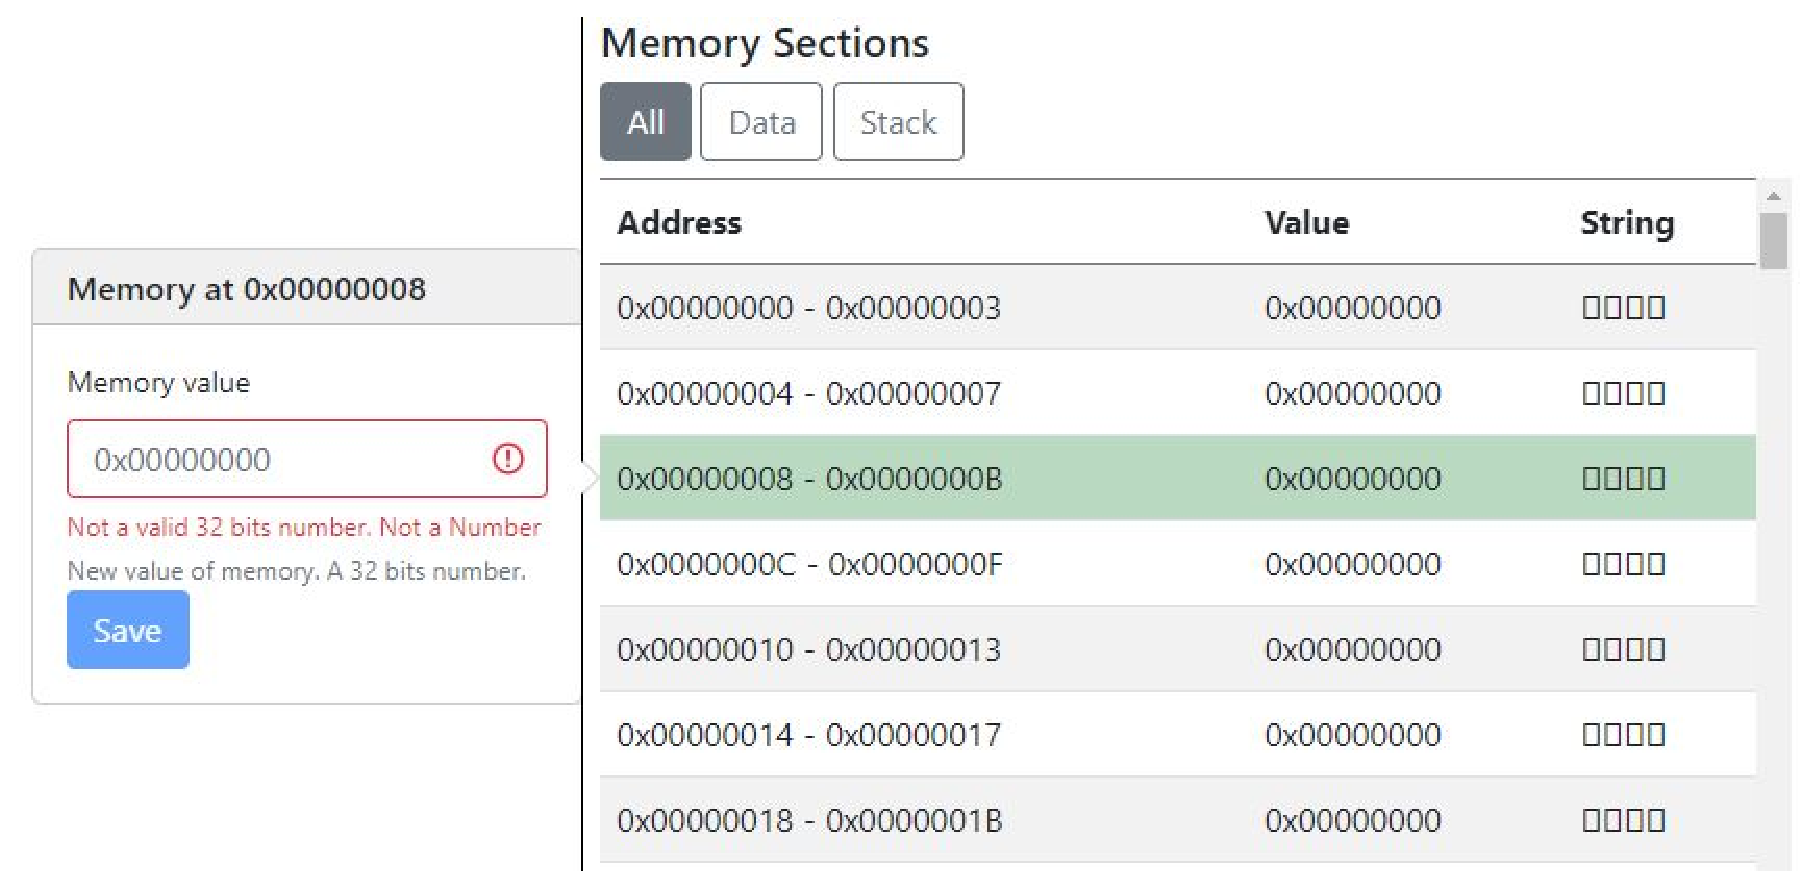
\includegraphics[width=0.85\textwidth]{images/modifymemory}
                \caption{Change Memory Value}
            \end{figure}

            \begin{figure}[h]
                \centering
                \includegraphics[width=0.85\textwidth]{images/stack}
                \caption{Stack Example}
            \end{figure}            
        }
    }

\section{Conclusiones}
{
}

\section{Bibliografía}
{
}

\end{document}